

\chapter{System architecture}
This chapter presents the description of the architecture of the embedded electronics subsystems on both DORIS and remote control base. The architecture is divided into subparts of interest in order to facilitate the understanding of both overall system and detailed subsystems.


\section{DORIS overall system}
As described in mechanics project, DORIS is composed by interconnected mobile modules, and each one is responsible for specific functions to achieve the main objective of this project: monitor, inspect and supervise the operation of a generic offshore facility. The modules resemble connected wagons moving along a rail installed throughout the facility, and each "wagon" carries specific devices to perform specific functions.
\newline
There are four different modules in this project:
\begin{itemize}
  \item Traction module (module \#1)
  \begin{itemize}
    \item This module is responsible for the traction of all modules along the rail, including itself. Besides all mechanic parts, it carries electric motors, power drivers for their control and other electronic circuits.
  \end{itemize}
  \item Power supply module (module \#2)
  \begin{itemize}
    \item This module is responsible for the power supply of the electronics system of all modules, including itself. Besides all mechanic parts, it carries battery packs, circuits for battery management, circuits for the system startup/shutdown, emergency system, radio and other electronic circuits.
  \end{itemize}
  \item Manipulator module (module \#3)
  \begin{itemize}
    \item This module contains the manipulator of the robot, a computer, a data acquisition system (DAQ) and few sensors.
  \end{itemize}
  \item Signal processing module (module \#4)
  \begin{itemize}
    \item This module contains a powerful computer for heavy processing, cameras, microphones and devices for wireless interface.
  \end{itemize}
\end{itemize}
These modules can be interconnected in any order. Considering a simple system using only one unit of each module type (basic system), the most recommendable module arrangement would be the described above because:
\begin{itemize}
  \item Power supply and signal processing modules are heavier. These module configuration balances the total robot weight.
  \item The system traction have better performance if the traction module is placed ahead the other modules, pulling the robot.
  \item Video and audio capture can be taken in a wider area if cameras and microphones are allocated in/on end modules.
\end{itemize}
All modules, regardless of how many will compose DORIS, are interconnected by: a) a Ethernet Network; b) a Controller Area Network (CAN); c) power cables. This means that all electronic devices in all modules are interconnected. In addition, an Wi-Fi access point located on the signal processing modules ensure a fast communication between the robot Ethernet system and a remote control base fixed at some point on the offshore facility.
\newline
The following subsections describes in detail each part of interest within DORIS electronics system.

\subsection{Communications diagram}
The following diagram (Figure~\ref{FIG:DESIGNEDCOMDIAGRAM}) describes the communications of the overall DORIS electronics system that was designed.
\begin{figure}
  \centering
  % Requires \usepackage{graphicx}
  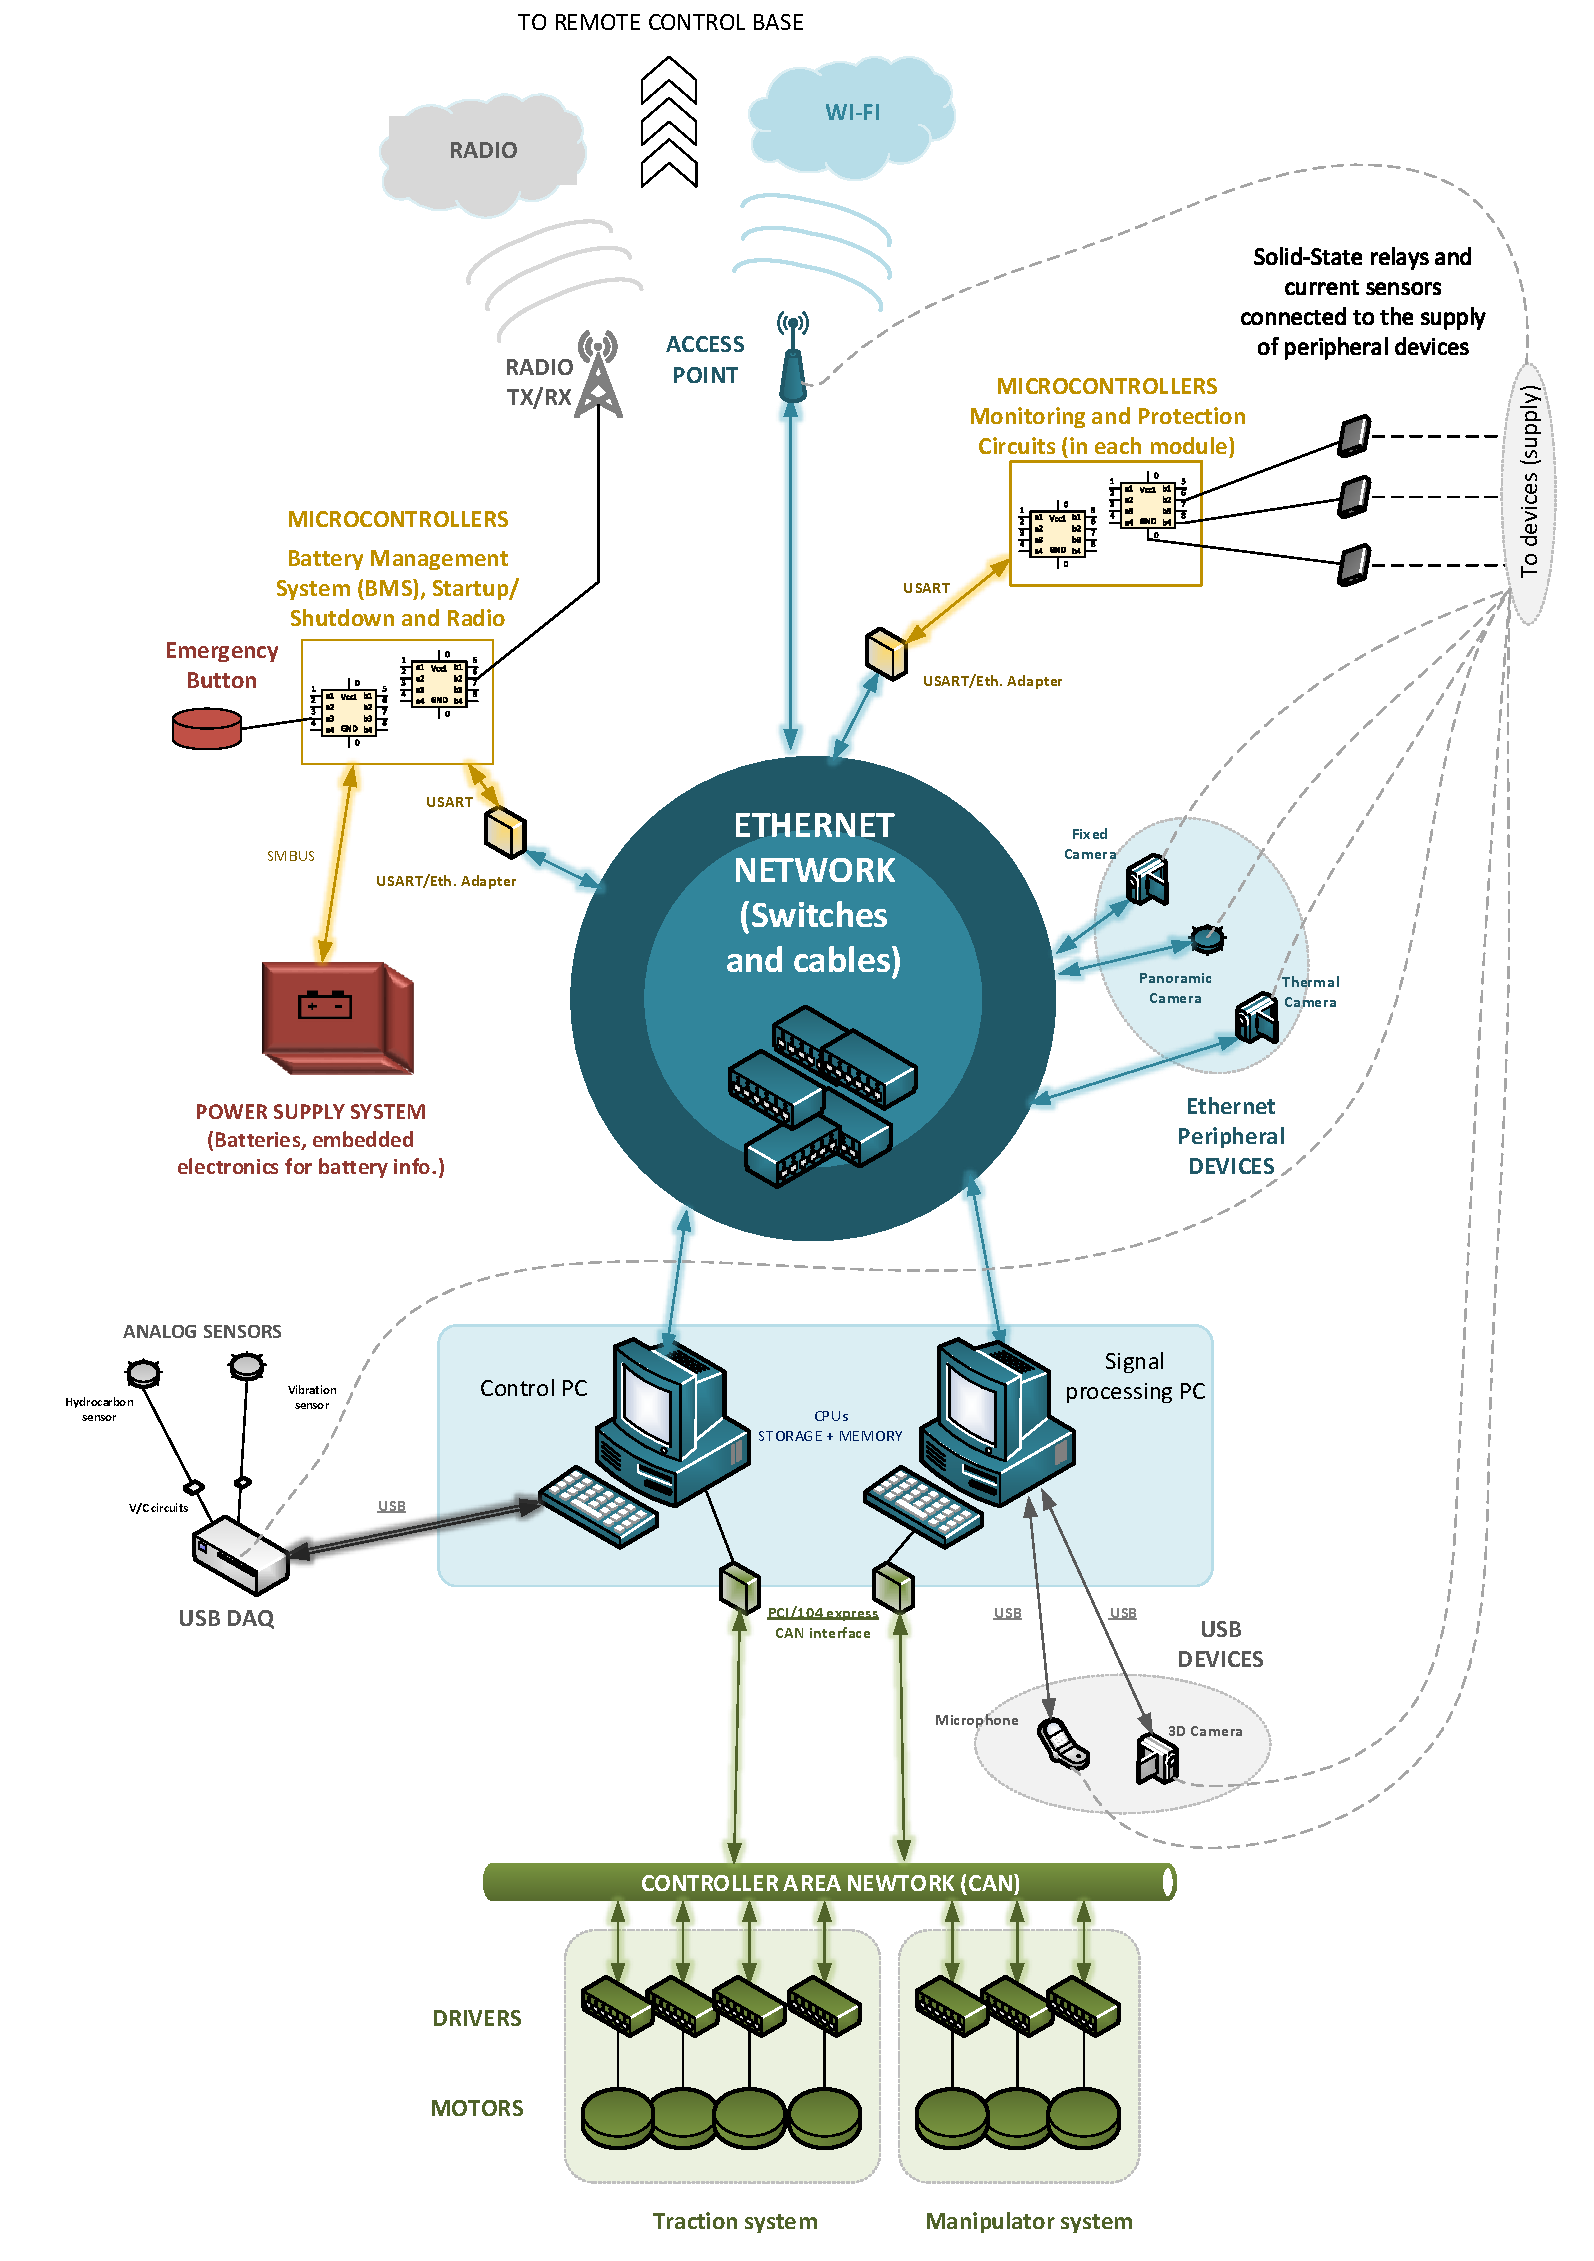
\includegraphics[angle=90,width=1\columnwidth]{figs/body01/FIGDESIGNEDCOMDIAGRAM.pdf}\\
  \caption[Overall communications diagram of the designed system]{Overall communications diagram of the designed system}
  \label{FIG:DESIGNEDCOMDIAGRAM}
\end{figure}
However, in practice, DORIS electronic system is flexible and can rely on expansions, such as:
\begin{itemize}
  \item Addition of new modules.
  \item Reconfiguration of modules order.
  \item Addition of new peripheral devices, as long as they are compatible with the system available interfaces, software/driver, and meet size and weight requirements from mechanical project.
\end{itemize}
Thus, the following diagram (Figure~\ref{FIG:EXPANSIONSCOMDIAGRAM}) describes the communications of the overall DORIS electronics system considering its possible expansions.
\begin{figure}
  \centering
  % Requires \usepackage{graphicx}
  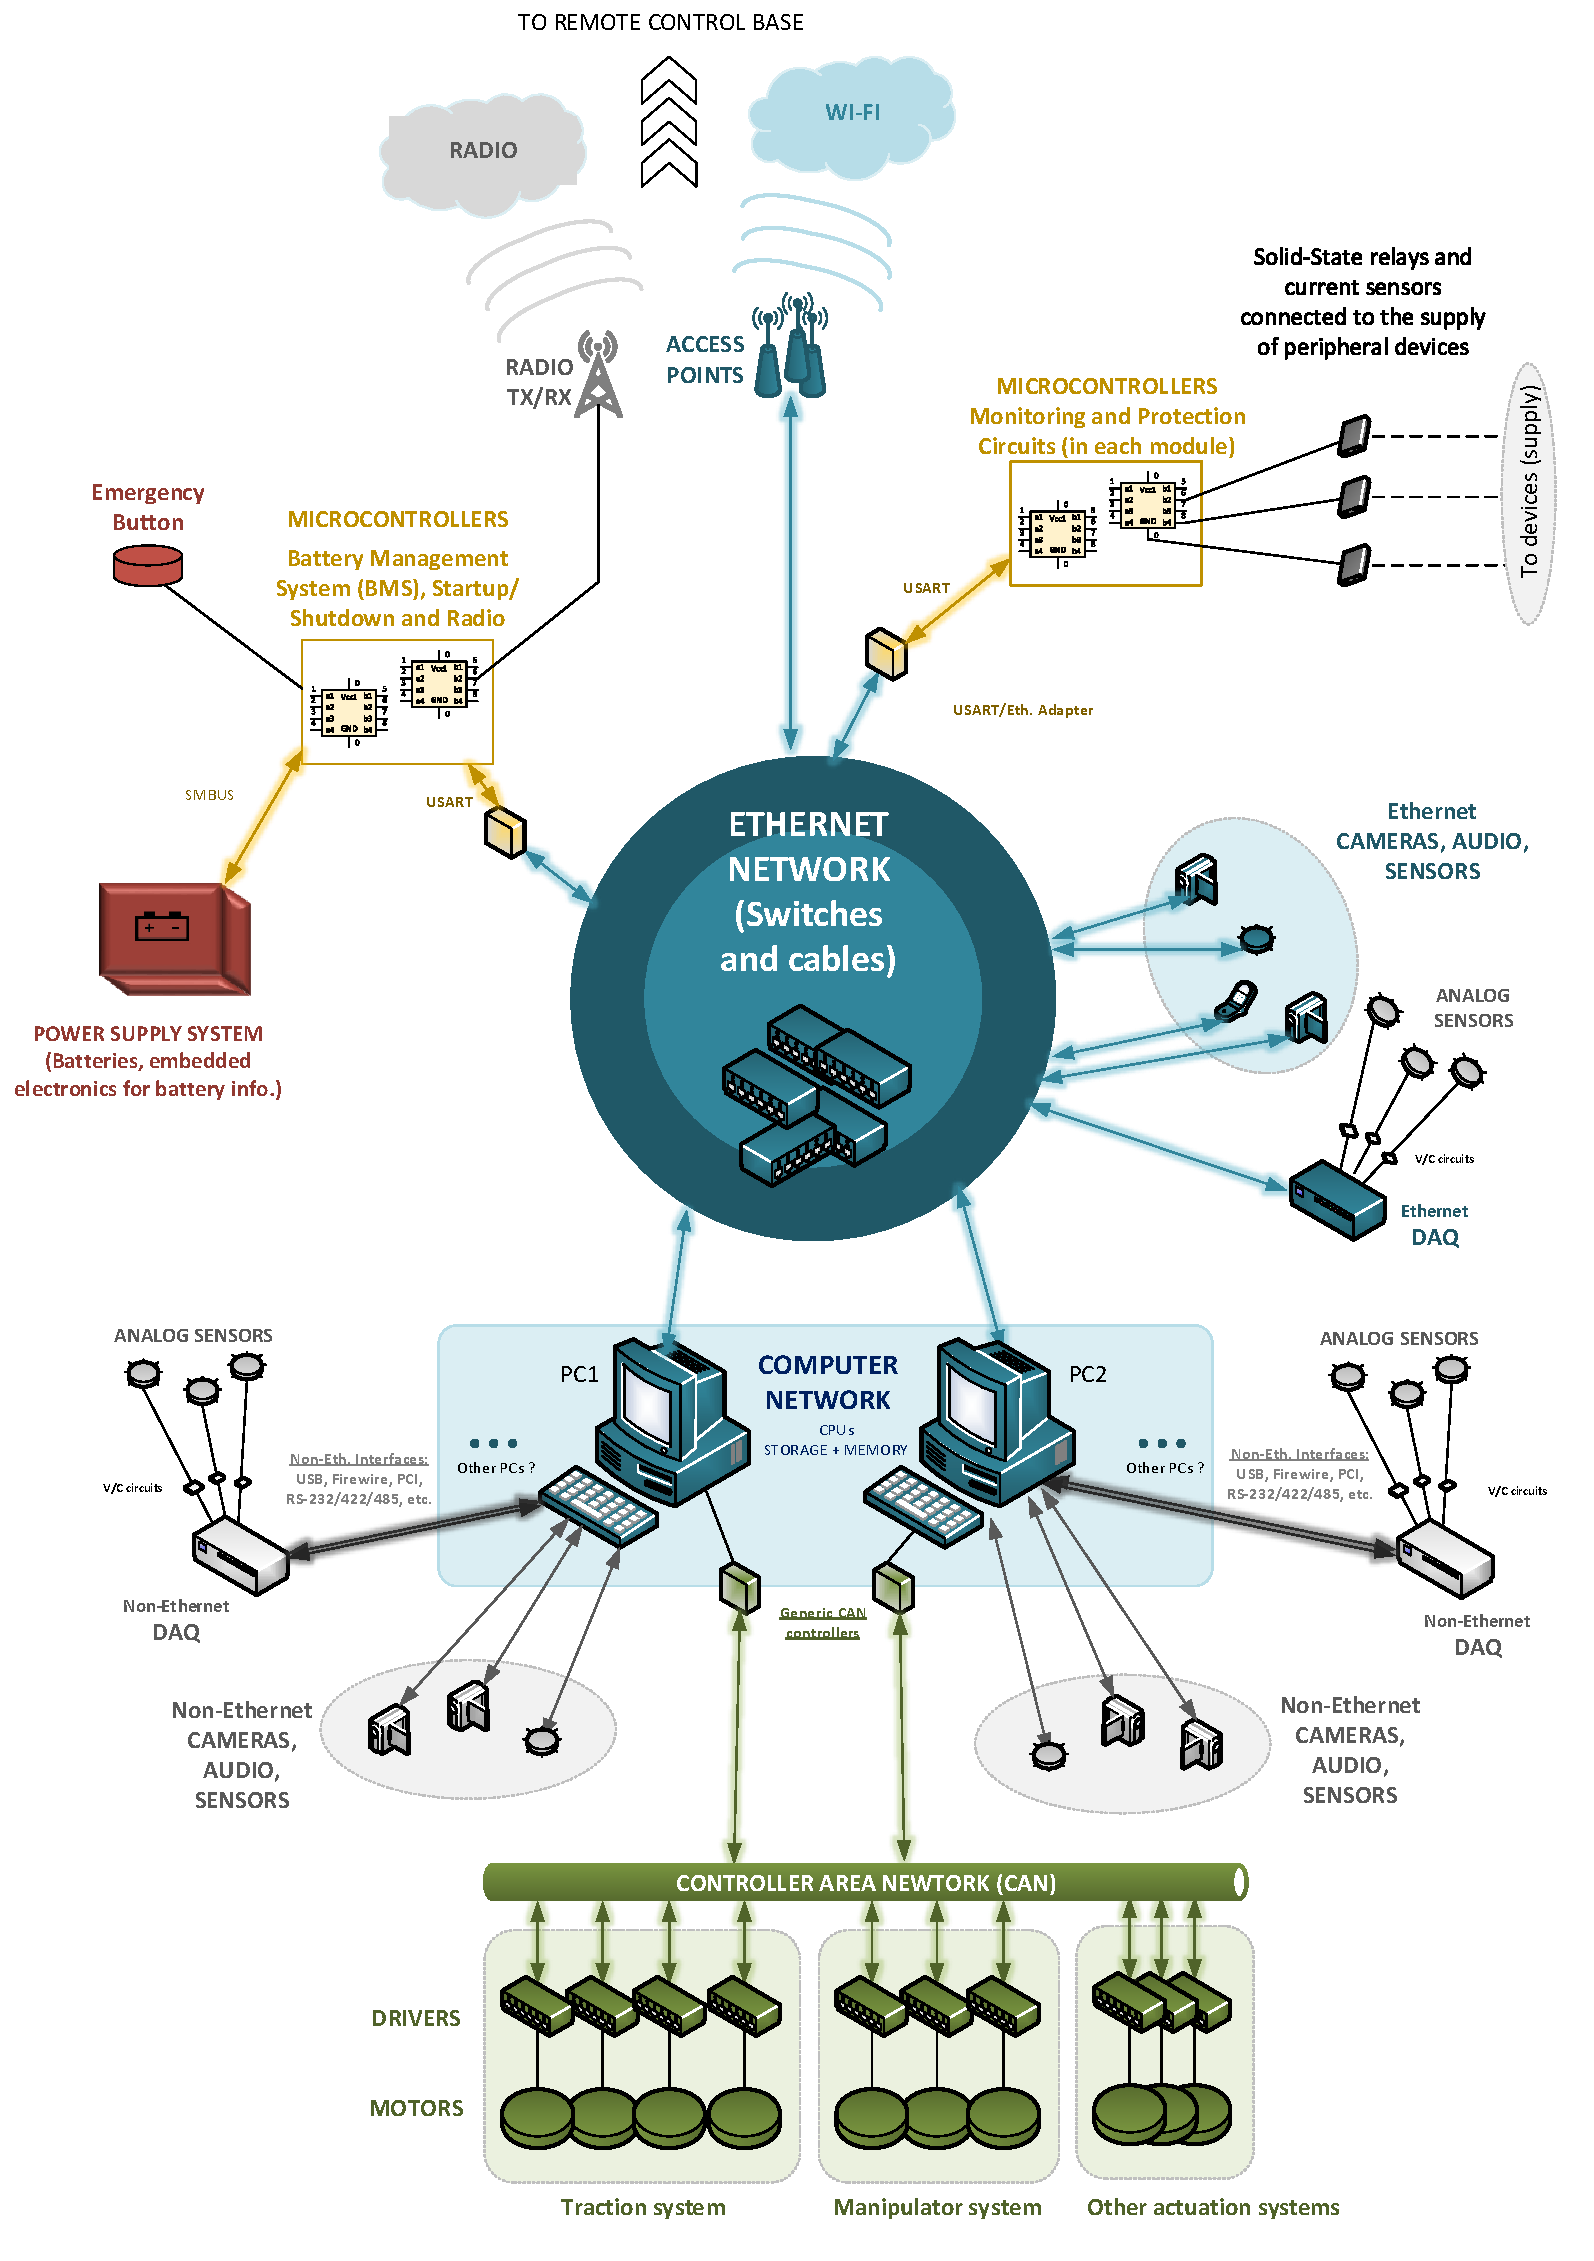
\includegraphics[angle=90,width=1\columnwidth]{figs/body01/FIGEXPANSIONSCOMDIAGRAM.pdf}\\
  \caption[Overall communications diagram considering system expansions]{Overall communications diagram considering system expansions}
  \label{FIG:EXPANSIONSCOMDIAGRAM}
\end{figure}

\subsection{Module diagram}
The following diagrams describe the system architecture inside each module type, not considering any expansion.

\subsubsection{Traction module diagram: Module \#1}
\subsubsection{Power supply module diagram: Module \#2}
\subsubsection{Manipulator module diagram: Module \#3}
\subsubsection{Signal processing module diagram: Module \#4}

\section{Computers}
DORIS basic system is composed by two computers.

\subsubsection{Control PC}
Control PC description:
  \begin{itemize}
    \item Main function: control DORIS motors. Thus, it controls both traction system and manipulator.
    \item Secondary functions: a) mission control management; b) navigation; c) input for data acquisition system; d) data transmission.
    \item Running software: this PC runs ROS (Ubuntu-Linux based software).
    \item Location: manipulator module (\#3).
    \item Model: ADL (manufacturer) ADLQM67PC-2715QE (model). For more details, see section~\ref{DEVICE:PC}.
    \item Accessories:
    \begin{itemize}
      \item CAN controller. PEAK (manufacturer) CAN Interface for PCI/104-Express IPEH-003057 (model).
      \item ESCREVER SSD
      \item ESCREVER
    \end{itemize}
    \item The computer and the storage card (Solid-State Drive) are both supplied by 5VDC and 12VDC, which are available at DORIS power buses (see G3 project).
  \end{itemize}
The following diagram (Figure~\ref{FIG:CONTROLPCDIAGRAM}) shows the control PC and its main interfaces and connections.
%\begin{figure}
%  \centering
%  % Requires \usepackage{graphicx}
%  \includegraphics[angle=90,width=1\columnwidth]{figs/body01/NEWBLOCKDIAGRAM.pdf}\\
%  \caption[Control PC interfaces and connections]{Control PC interfaces and connections}
%  \label{FIG:CONTROLPCDIAGRAM}
%\end{figure}

\subsubsection{Signal processing PC}
Signal processing PC description:
  \begin{itemize}
    \item Main function: signal processing. Thus, this PC: a) receives audio and video data from all cameras, microphones and sensors; b) runs signal processing and compression algorithms developed by G5 team.
    \item Secondary function: data transmission. Thus, this PC can transmit the processed/compressed data to DORIS local network and, hence, to the remote base via Wi-Fi.
    \item Running software: this PC runs ROS (Ubuntu-Linux based software).
    \item Location: signal processing module (\#4).
    \item Model: ADL (manufacturer) ADLQM67PC-2715QE (model). For more details, see section~\ref{DEVICE:PC}.
    \item Accessories:
    \begin{itemize}
      \item CAN controller. PEAK (manufacturer) CAN Interface for PCI/104-Express IPEH-003057 (model).
      \item ESCREVER SSD
      \item ESCREVER
    \end{itemize}
    \item The computer and the storage card (Solid-State Drive) are both supplied by 5VDC and 12VDC, which are available at DORIS power buses (see G3 project).
  \end{itemize}
The following diagram (Figure~\ref{FIG:SIGNALPROCESSINGPCDIAGRAM}) shows the signal processing PC and its main interfaces and connections.
%\begin{figure}
%  \centering
%  % Requires \usepackage{graphicx}
%  \includegraphics[angle=90,width=1\columnwidth]{figs/body01/NEWBLOCKDIAGRAM.pdf}\\
%  \caption[Signal processing PC interfaces and connections]{Signal processing PC interfaces and connections}
%  \label{FIG:SIGNALPROCESSINGPCDIAGRAM}
%\end{figure}

\section{Video, audio and sensor devices}
ESCREVER

\section{Local Area Network (LAN)}
The system have a main local area network (LAN), which is responsible for most of the data traffic flowing through all modules and between DORIS and the remote control base. The LAN physical layer inside DORIS is Ethernet based, whereas the LAN physical layer between DORIS and the base is Wi-Fi based. The following diagram (Figure~\ref{FIG:LANDIAGRAM}) depicts the overall system LAN.
\begin{figure}
  \centering
  % Requires \usepackage{graphicx}
  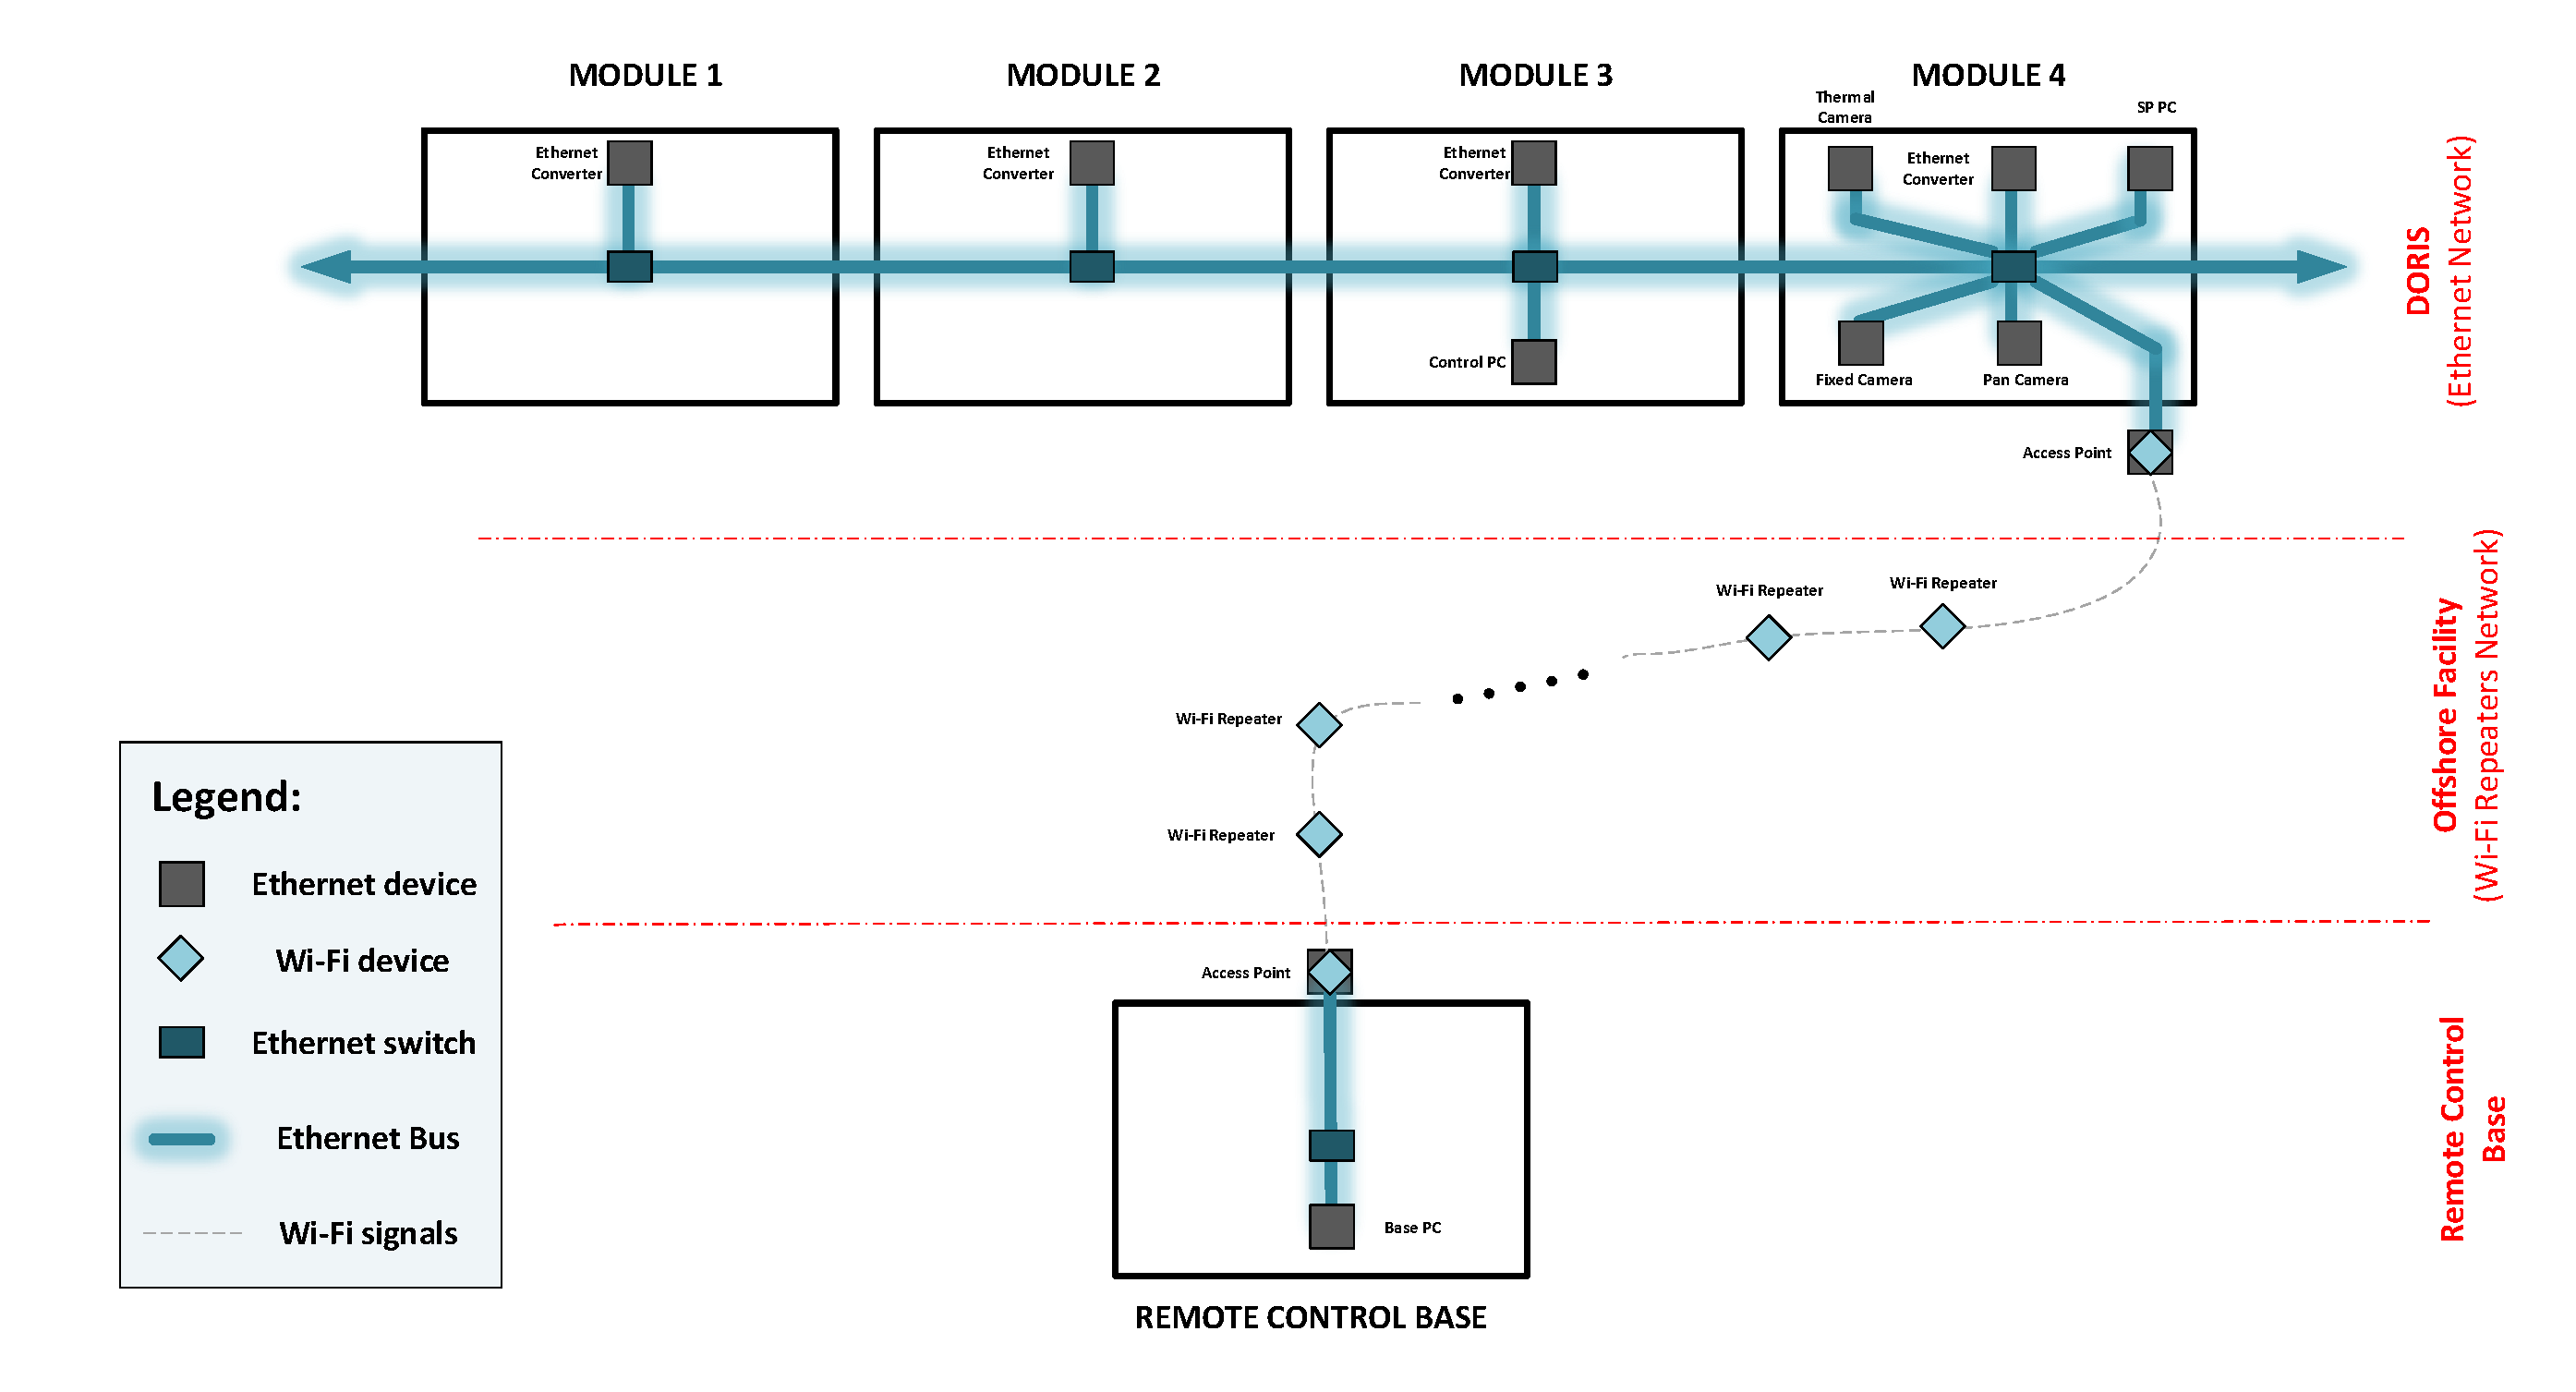
\includegraphics[angle=90,width=1\columnwidth]{figs/body01/FIGLANDIAGRAM.pdf}\\
  \caption[Local Area Network - Overall architecture]{Local Area Network - Overall architecture}
  \label{FIG:LANDIAGRAM}
\end{figure}

\subsection{Ethernet communication}
DORIS local area network is Gigabit Ethernet (IEEE 802.3-2005) based. The structure of DORIS Ethernet network has the following features:
\begin{itemize}
  \item Each module has two Ethernet outputs: front and rear.
  \item Each module contains an Ethernet Switch, which joins the Ethernet bus inside the module and extends the Ethernet network to other peripheral devices.
  \item Traction and power supply modules contain a 5-Gigabit port Ethernet Switch. Manufacturer: Korenix. Model: 3005G. For more details, see section~\ref{DEVICE:ETHERNETSWITCH3005G}.
  \item Manipulator and signal processing modules require more ports due to the great number of peripheral devices on them. Each of them contains a 8-Gigabit port Ethernet Switch. Manufacturer: Korenix. Model: 3008G. For more details, see section~\ref{DEVICE:ETHERNETSWITCH3008G}.
  \item All four Ethernet switches are supplied by 24VDC, which is available at DORIS power buses (see G3 project).
  \item Independently of the chosen DORIS module arrangement, there will be always an Ethernet bus passing through all modules.
  \item The Ethernet cables inside the modules are all flexible and shielded CAT.5e, 6 or 7 standard (see model in section~\ref{DEVICE:ETHERNETINCABLES})
  \item The Ethernet cables outside modules are all flexible and shielded CAT.5e, 6 or 7 standard (see model in section~\ref{DEVICE:ETHERNETOUTCABLES}). These outdoor cables must be more flexible and resistent to meet mechanical requirements, such as: resistance against stress, water, chemicals, heat and non-release of toxic fumes in case of fire.
  \item All Ethernet cables and connectors can be checked in sections~\ref{DEVICE:CABLELIST} and~\ref{DEVICE:CONNECTORLIST}.
\end{itemize}
The following diagram (Figure~\ref{FIG:ETHERNETDIAGRAM}) depicts DORIS Ethernet network.
\begin{figure}
  \centering
  % Requires \usepackage{graphicx}
  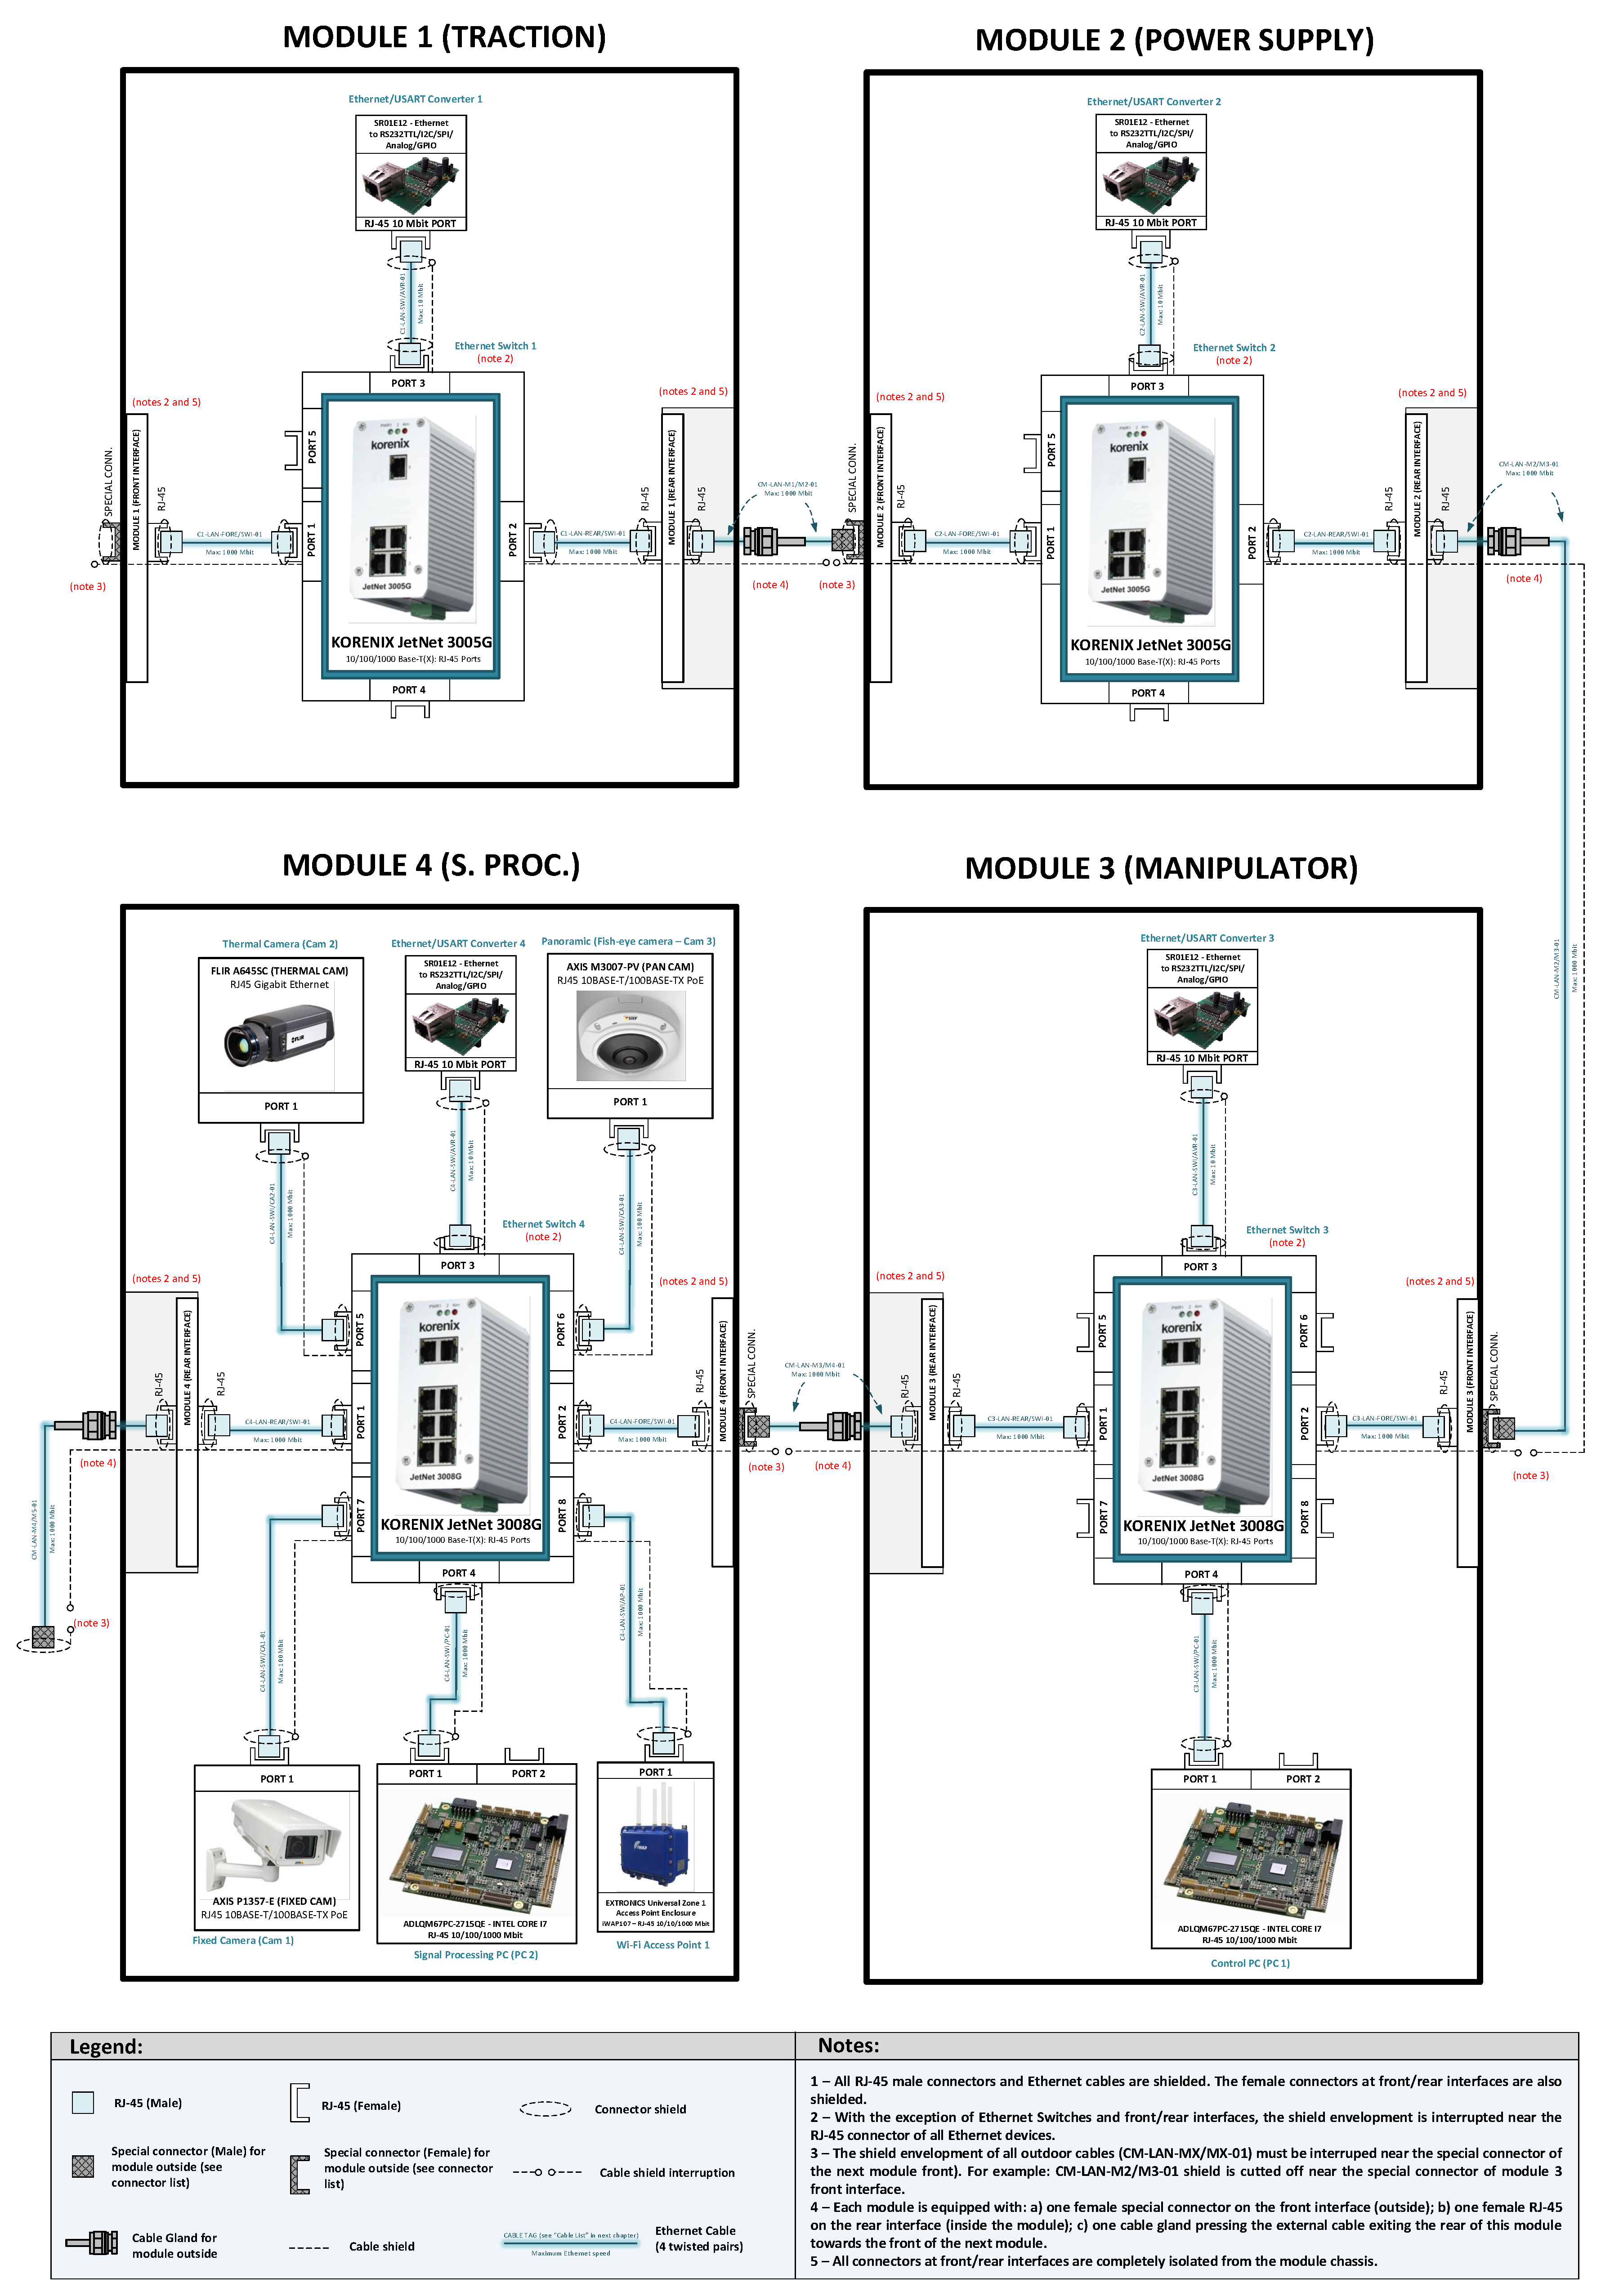
\includegraphics[angle=90,width=1\columnwidth]{figs/body01/FIGETHERNETDIAGRAM.pdf}\\
  \caption[DORIS Ethernet Network - Detailed architecture]{DORIS Ethernet Network - Detailed architecture}
  \label{FIG:ETHERNETDIAGRAM}
\end{figure}
\subsection{Wi-Fi communication}
The system Wi-Fi network follows IEEE 802.11n standard, which means that data transmission via Wi-Fi can reach a 300Mbps baud rate. The structure of the system Wi-Fi network has the following features:
\begin{itemize}
  \item An Access Point located on DORIS signal processing module (\#4), connected to one port of the respective Ethernet switch.
  \item An Access Point located on the remote control base (the remote control base project is detailed further, in section~\ref{REMOTECONTROLBASE}.
  \item Wi-Fi repeaters distributed over specific point on the offshore facility. The repeater network topology may vary with the structure of each facility type.
  \item DORIS Access Point is supplied by 24VDC, which is available at DORIS power buses (see G3 project).
  \item The remote control base Access Point is supplied by 24VDC, which is available at the facility (ESCREVER).
  \item Repeaters must receive electric power from the available electric structure at the facility.
  \item The Access Point model is iWAP107 (Manufacturer: Extronics). It is equipped with the antenna ESCREVER. For more details, see sections~\ref{DEVICE:WIFIACCESSPOINT} and~\ref{DEVICE:WIFIANTENNA}.
  \item The repeater model is ESCREVER. For more details, see section~\ref{DEVICE:WIFIREPEATER}.
  \item Since Wi-Fi is a wireless mean of transmission, it must comply with the requirements for safe operation of RF (Radio Frequency) signals in hazardous areas (which is the case of any offshore facility). In most circumstances, low-power radios operating at less then 100mW EIRP (Equivalent Isotropically Radiated Power) and 2.4 and 5.8 GHz do not offer any risk under normal circumstances. Nevertheless, we strongly recommend that the facility's safety administration is consulted beforehand to determine its policy on the use of RF devices. The are extremely low chances that RF interferences will lead to a safety problem or cause an accident by heating effect, but caution is always required.
  \item The specified Wi-Fi devices for this system are protected with:
      \begin{itemize}
        \item Explosion proof enclosure (Ex d compliant), which means that any possible ignition caused by device circuits will be contained in the enclosure and not come into contact with the explosive atmosphere. Since there are many different classifications for a hazardous area (Zones, Groups, Div., see ESCREVER for more information)
        \item Intrinsically safe RF outputs (Ex i). This means that the antenna output power meets the safety parameters of the barrier and the RF EIRP allowed limitations in hazardous areas. For more information, see ESCREVER.
        \item The Wi-Fi system must comply with ESCREVER standards. See ESCREVER.
      \end{itemize}
\end{itemize}
The following diagram (Figure~\ref{FIG:WIFIDIAGRAM}) depicts Wi-Fi system network.
%\begin{figure}
%  \centering
%  % Requires \usepackage{graphicx}
%  \includegraphics[angle=90,width=1\columnwidth]{figs/body01/FIGWIFIDIAGRAM.pdf}\\
%  \caption[System Wi-Fi Network - Detailed architecture]{System Wi-Fi Network - Detailed architecture}
%  \label{FIG:WIFIDIAGRAM}
%\end{figure}
\section{Actuation system}
DORIS actuation system is responsible for the control of two DORIS subsystems: traction and manipulator. These two subsystem are controlled by DORIS computers via Controller Area Network-CAN (see section~\ref{CANDESCRIPTION} for more details). The following diagram (Figure~\ref{FIG:OVERALLACTDIAGRAM}) summarizes the overall actuation system and its subsystems:

\begin{figure}
  \centering
  % Requires \usepackage{graphicx}
  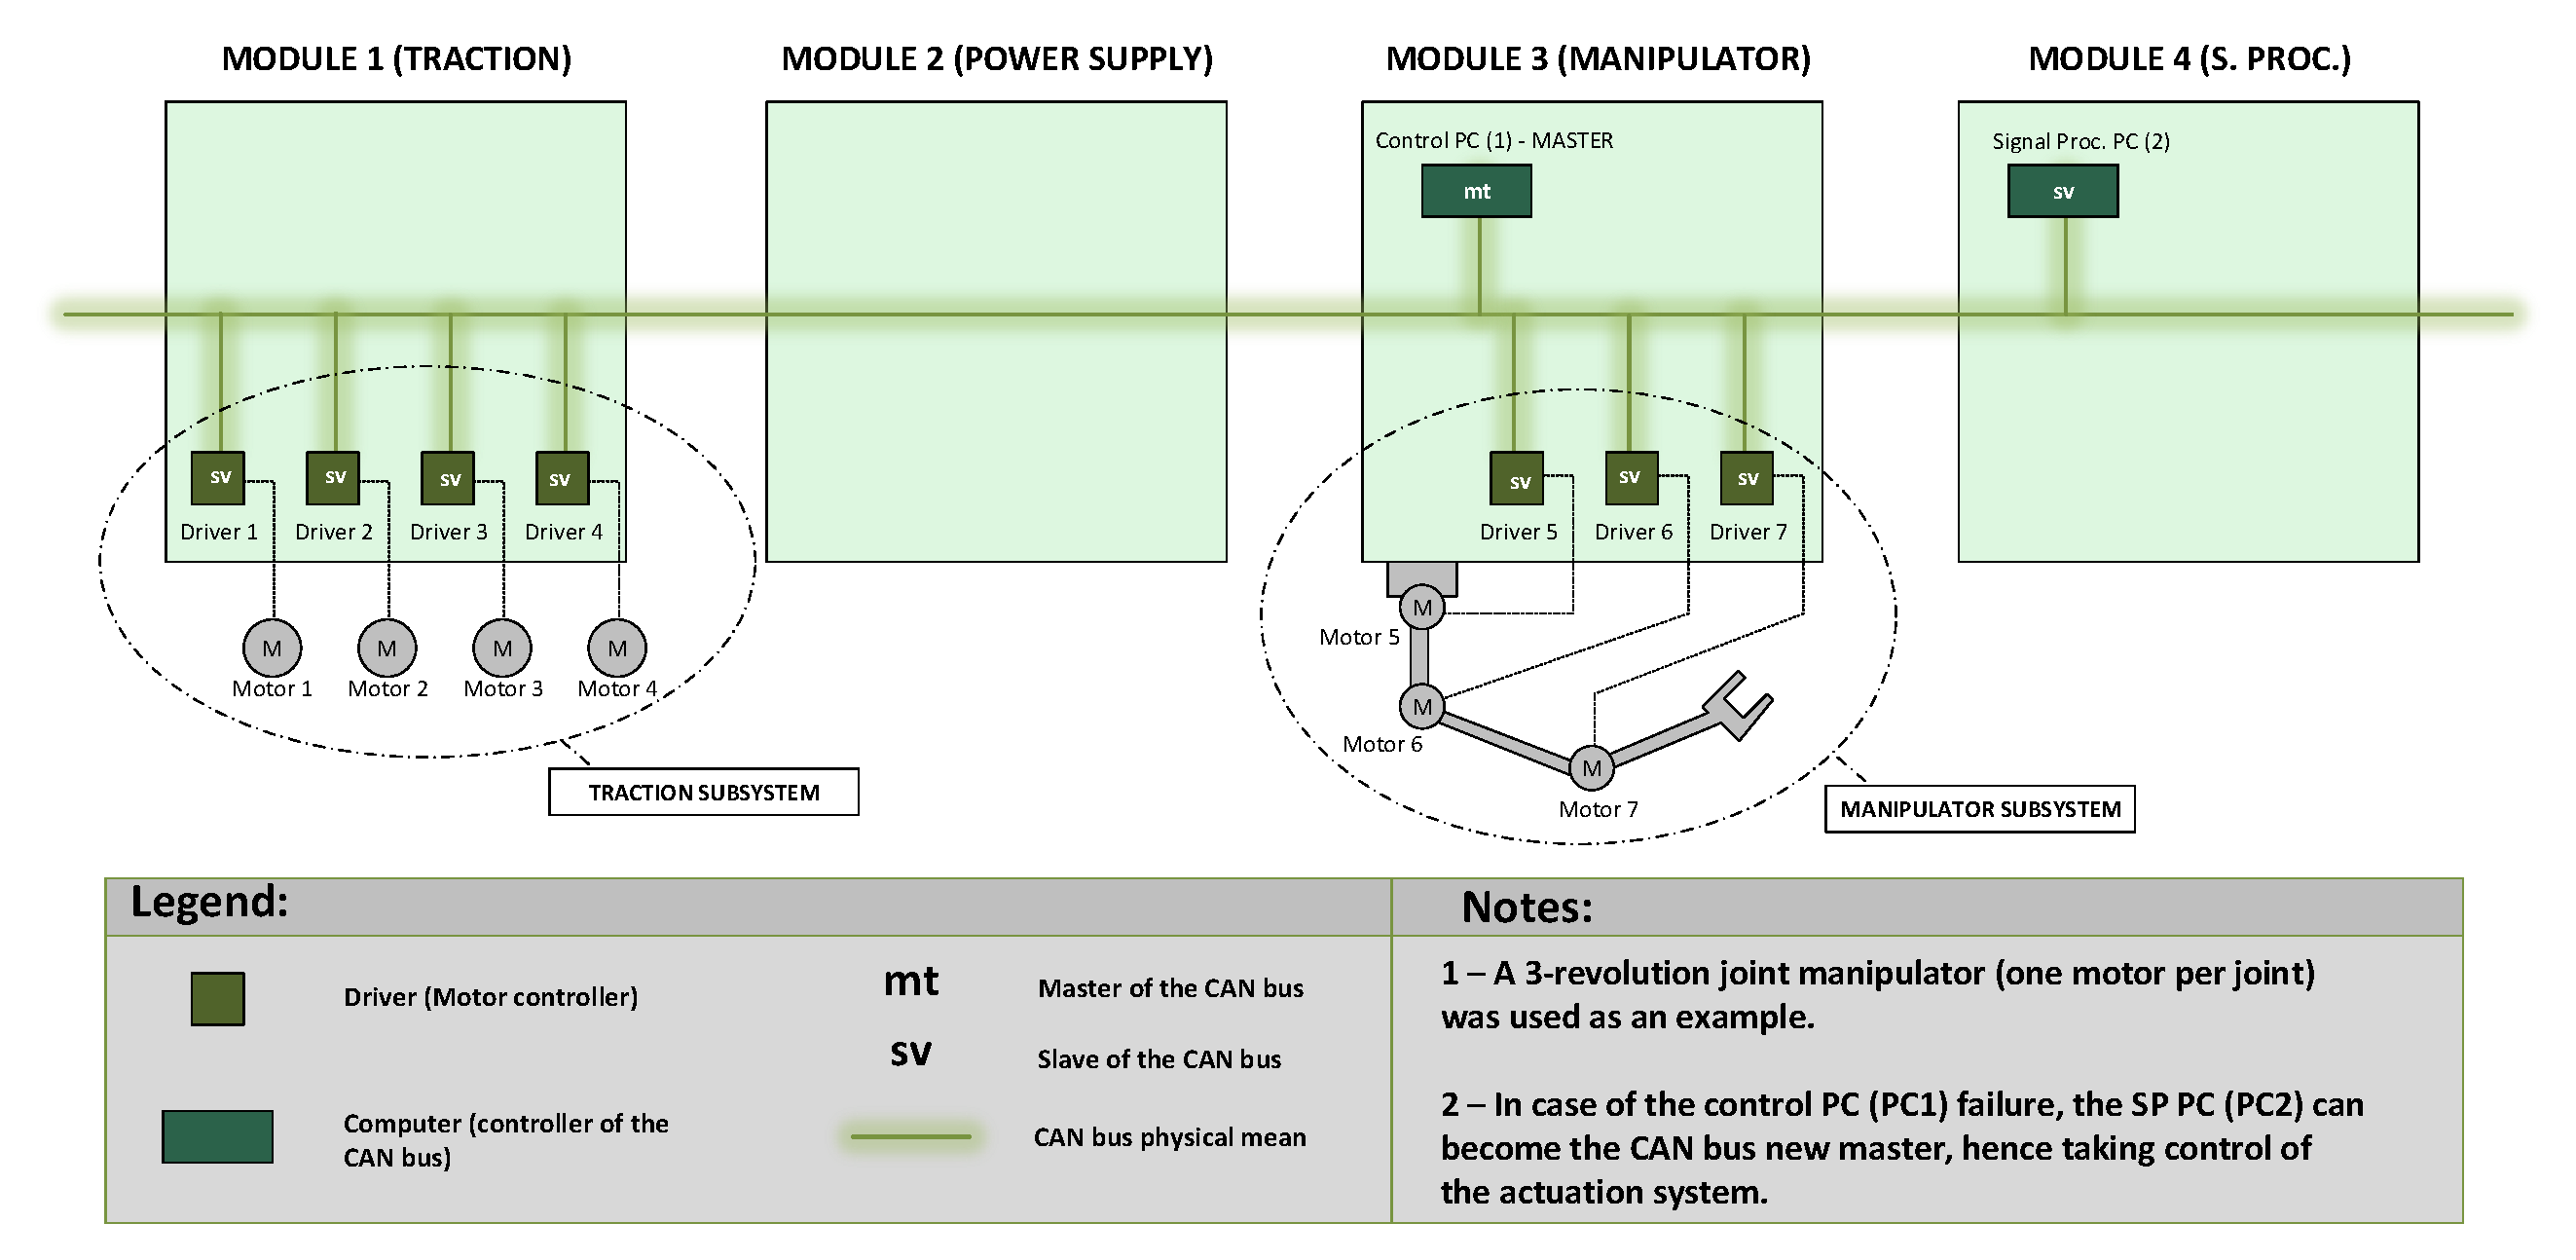
\includegraphics[angle=90,width=1\columnwidth]{figs/body01/FIGOVERALLACTDIAGRAM.pdf}\\
  \caption[Overall actuation system diagram and traction/manipulator subsystems]{Overall actuation system diagram and traction/manipulator subsystems}
  \label{FIG:OVERALLACTDIAGRAM}
\end{figure}

\subsection{Traction subsystem}
DORIS traction system is responsible for its movement along the rail installed in the facility. As mentioned before, the traction system is part of the Traction module (\#1). The electronics of the traction system is composed by:
\begin{itemize}
  \item 4x (four) actuator combinations by Maxon Motor (Part Number: 470625), each containing:
  \begin{itemize}
    \item One EC brushless electric motor. Model: Maxon Motor EC-4pole 30 diam. 30 mm, brushless, 200 Watt High Power, Part Number: 305013 (for more details, see ESCREVER).
    \item One reduction gear (reduction of 299/14). Model: Maxon Motor Planetary Gearhead GP 32 HP diam. 32 mm, 4.0-8.0 Nm, Metal Version, High Power, Part Number: 326660 (for more details, see ESCREVER).
    \item One encoder installed at motor base (not in the gear). Model: Encoder MR, Type ML, 500 CPT, 3 Channels, with Line Driver, Part Number: 225778 (for more details, see ESCREVER).
  \end{itemize}
  \item 4x Power Drivers for each motor control. Model: Maxon Motor EPOS2 70/10, Digital positioning controller, 10 A, 11-70 VDC, Part Number: 375711 (for more details, see ESCREVER).
  \item Cable set to connect (for more details, see ESCREVER):
  \begin{itemize}
    \item Each motor power (winding) to each driver.
    \item Each motor Hall effect sensor to each driver.
    \item Each motor encoder to each driver.
    \item Driver power supply and grounding.
    \item CAN connection between each driver.
    \item CAN connection between one driver and the rest of CAN network.
  \end{itemize}
  \item Connector set (for more details, see ESCREVER).
\end{itemize}

\subsection{Manipulator subsystem}
ESCREVER

\subsection{Controller Area Network (CAN) communication} \label{CANDESCRIPTION}
As mentioned, CAN is the chosen network standard to interconnect and control DORIS actuation system. This standard is distinguished for being suitable for real-time vehicle control applications involving sensors and actuators, with a strict error control.
\subsubsection{CAN physical layer}
CAN physical layer is composed by 4 channels:
\begin{itemize}
  \item CAN High
  \item CAN Low
  \item Ground (GND)
  \item Shield (SH)
\end{itemize}
All CAN data is transmitted using differential (balanced) signals, which means that a voltage difference is generated in CAN High and CAN Low at the transmitter, and the same voltage difference is recognized by the receiver. Both CAN High and Low are referenced to GND. Cables for CAN transmission must be shielded twisted pair. With this configuration, crosstalk effect is minimized. Noise interference is also minimized since the transmission is differential, i.e., any noise addition in one line will cause the same addition in another line, but the voltage difference remains the same. The shield channel is a protecting metallic mesh that envelops the other cable wires in order to block existing electromagnetic field on the environment and, hence, reduce interference.
\newline
Cables and connectors that compose CAN network are described in ESCREVER. For more information about CAN physical layer, see ESCREVER.
\subsubsection{DORIS CAN network and connections}
Independently of the chosen DORIS module arrangement, there will be always a CAN bus passing through all modules. The CAN bus has branches in all modules except for power supply module (\#2). The branches are:
\begin{itemize}
  \item In traction module (\#1): one branch to each traction motor driver.
  \item In manipulator module (\#3):
  \begin{itemize}
    \item One branch to the CAN controller, located on the control PC.
    \item One branch to each driver of the manipulator.
  \end{itemize}
  \item In signal processing module (\#4): one branch to the CAN controller, located on the signal processing PC.
\end{itemize}
With this configuration, either the control or the signal processing PC can be the master of CAN bus, and the other devices (other PC and drivers), the slaves. By default, the control PC is the bus master, but it can be changed by software, especially if any fault occurs in this PC.
\newline
The CAN interface at the drivers are very simple, because each driver is equipped with the needed hardware and software (CAN Open, see ESCREVER for more details). However, the computers are not equipped with CAN interfaces by themselves. A peripheral interface/expansion is needed. The chosen model fore the CAN interface is the product: PEAK CAN Interface for PCI/104-Express IPEH-003057 (see ESCREVER for more details). This CAN interface has the following features:
\begin{itemize}
  \item Compatible with PCI/104 express, which is the computer main data bus.
  \item Galvanic isolated dual channel CAN controller, which allows the control of two independent CAN buses (if needed) and electric isolation of between the bus and the computer, preventing ground current loops and common node noise (for more details about these problems, see ESCREVER and ESCREVER).
  \item Two male DB-9 connectors.
\end{itemize}
The following diagram (figure~\ref{FIG:DETAILEDCANDIAGRAM}) describes the detailed CAN bus architecture in DORIS:
%\begin{figure}
%  \centering
%  % Requires \usepackage{graphicx}
%  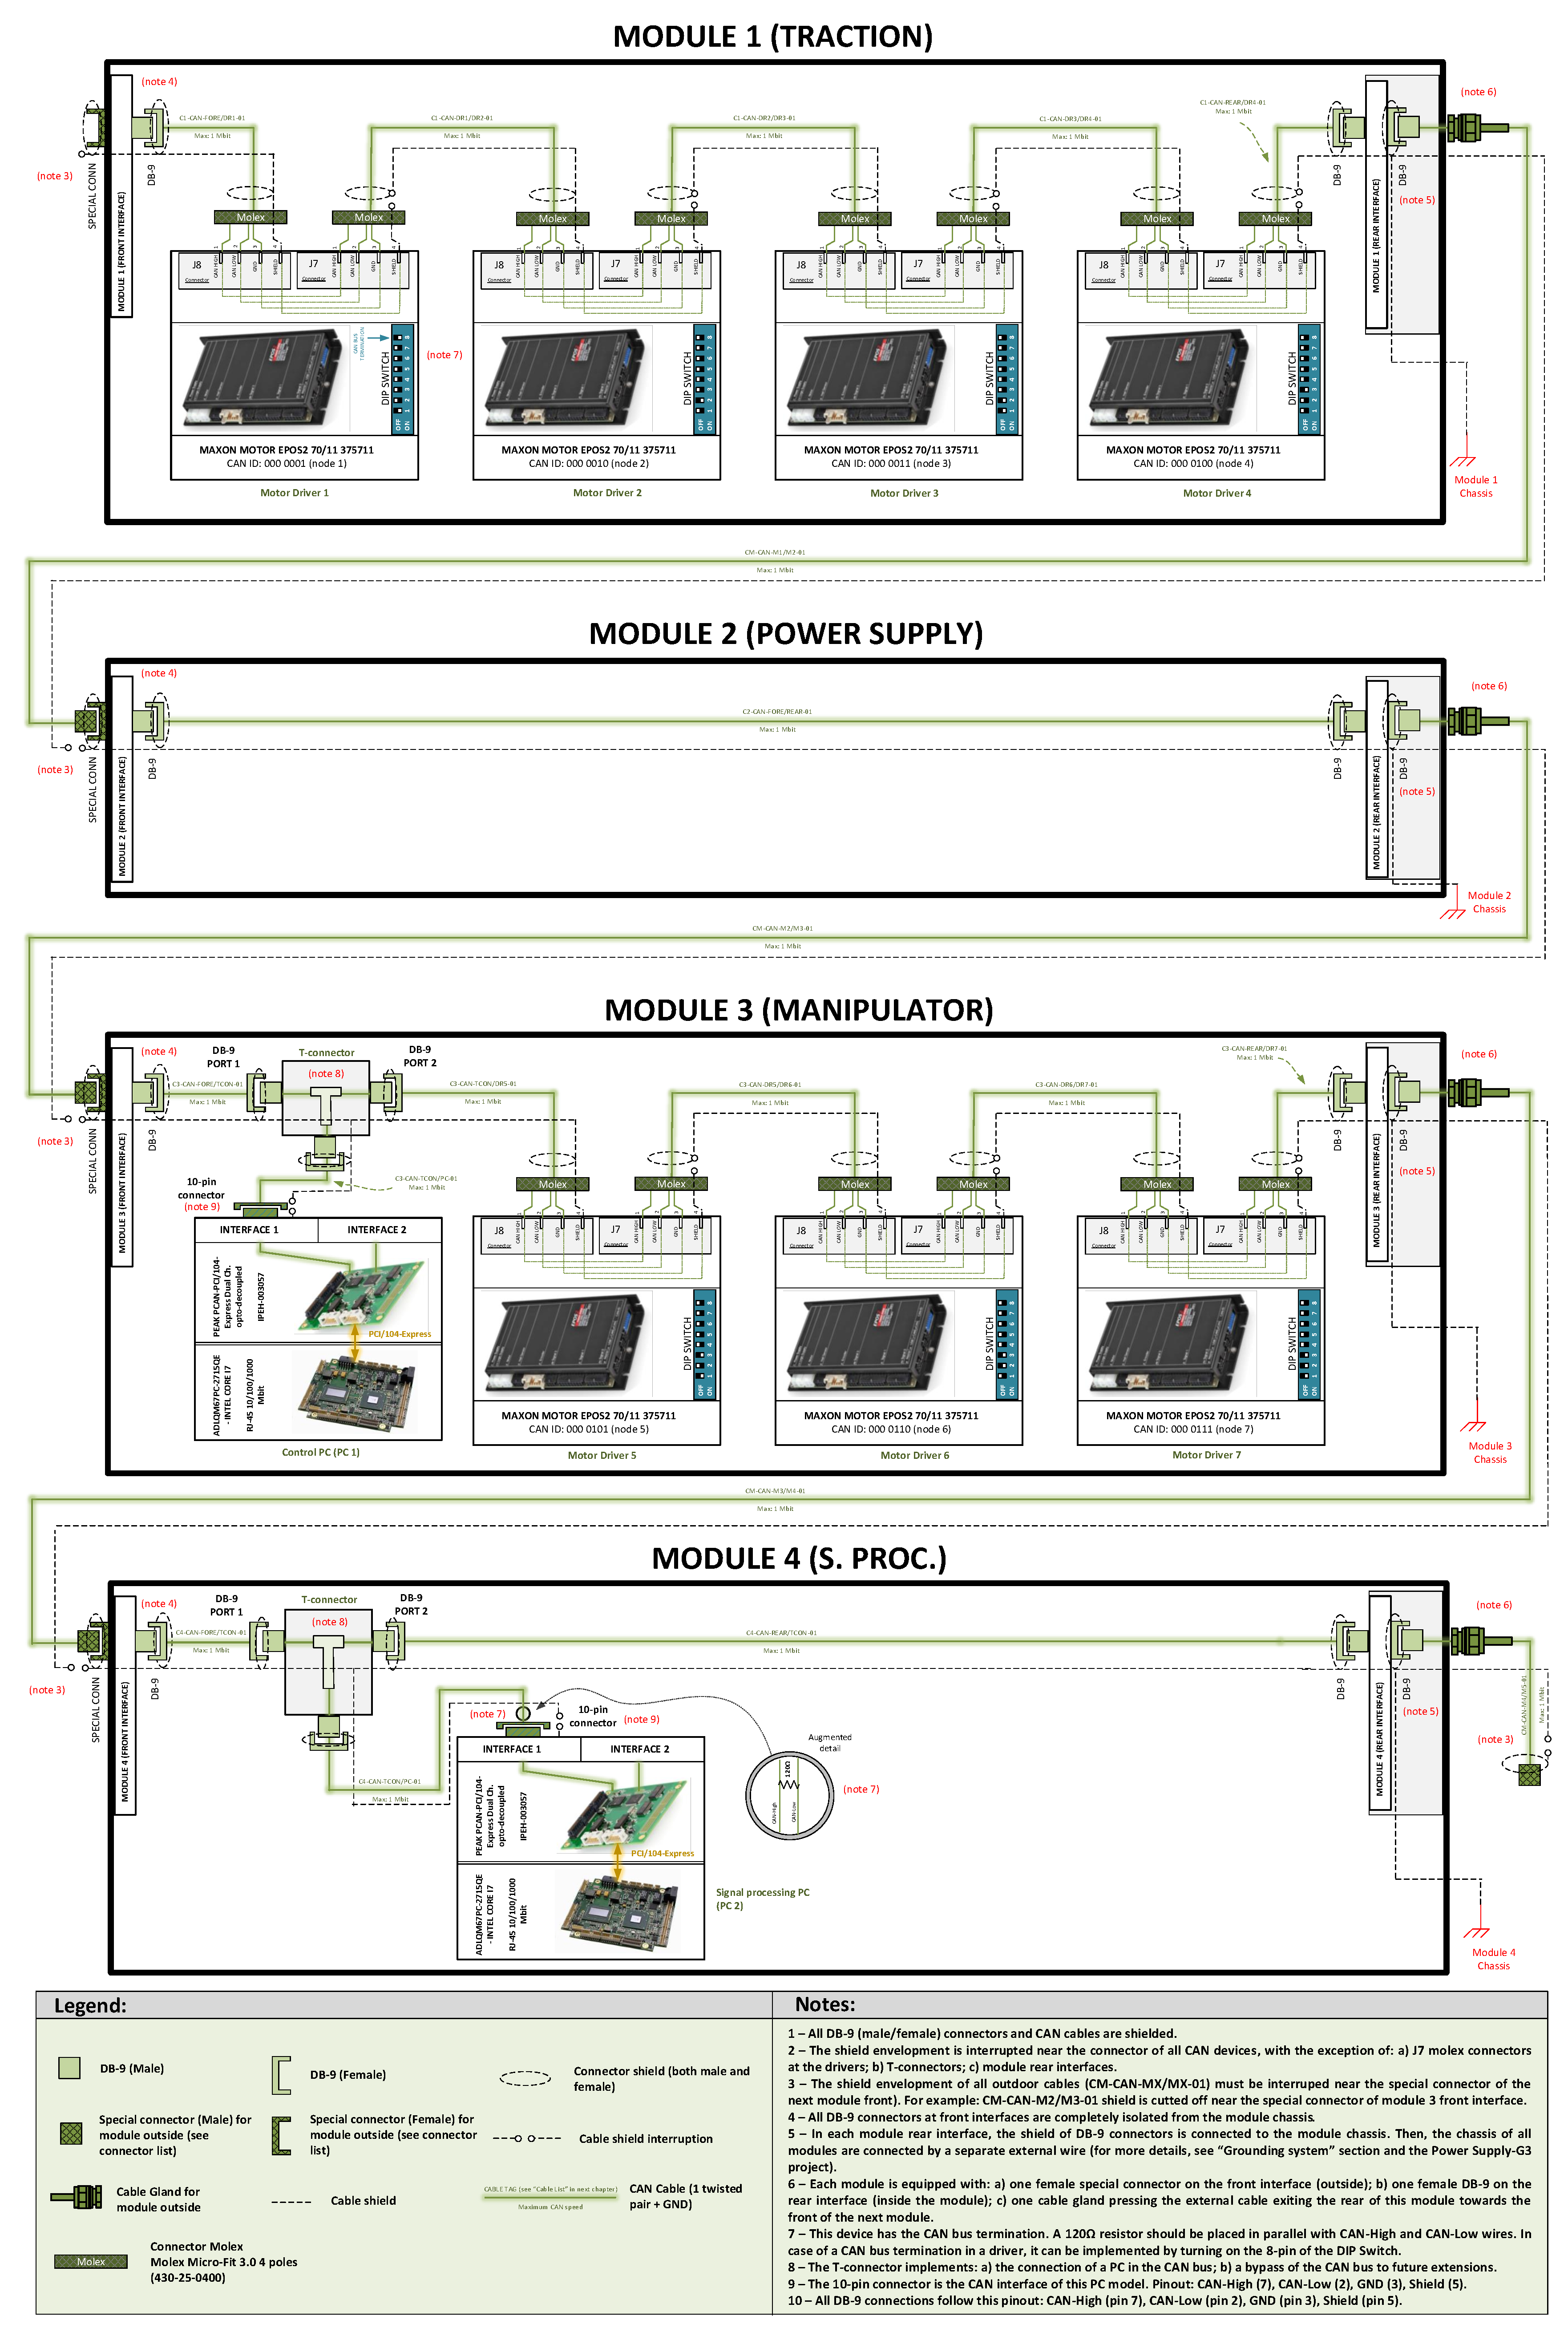
\includegraphics[angle=90,width=1\columnwidth]{figs/body01/FIGDETAILEDCANDIAGRAM.pdf}\\
%  \caption[Detailed CAN bus architecture]{Detailed CAN bus architecture}
%  \label{FIG:OVERALLCANDIAGRAM}
%\end{figure}
The following diagram (figure~\ref{FIG:CANTRACTIONDIAGRAM}) describes the CAN connections in traction module (\#1):
%\begin{figure}
%  \centering
%  % Requires \usepackage{graphicx}
%  \includegraphics[angle=90,width=1\columnwidth]{figs/body01/NEWBLOCKDIAGRAM.pdf}\\
%  \caption[CAN connections - Traction module (\#1)]{CAN connections - Traction module (\#1)}
%  \label{FIG:CANTRACTIONDIAGRAM}
%\end{figure}
The following diagram (figure~\ref{FIG:CANMANIPULATORDIAGRAM}) describes the CAN connections in manipulator module (\#3):
%\begin{figure}
%  \centering
%  % Requires \usepackage{graphicx}
%  \includegraphics[angle=90,width=1\columnwidth]{figs/body01/NEWBLOCKDIAGRAM.pdf}\\
%  \caption[CAN connections - Manipulator module (\#3)]{CAN connections - Manipulator module (\#3)}
%  \label{FIG:CANMANIPULATORDIAGRAM}
%\end{figure}
The following diagram (figure~\ref{FIG:CANSPDIAGRAM}) describes the CAN connections in signal processing module (\#4):
%\begin{figure}
%  \centering
%  % Requires \usepackage{graphicx}
%  \includegraphics[angle=90,width=1\columnwidth]{figs/body01/NEWBLOCKDIAGRAM.pdf}\\
%  \caption[CAN connections - Signal processing module (\#4)]{CAN connections - Signal processing module (\#4)}
%  \label{FIG:CANSPDIAGRAM}
%\end{figure}

\section{Supervisory circuits}
Figure~\ref{FIG:CANBUS1FIG} illustrates the actuator interfaces. The motors for both locomotion and manipulator are controlled by drivers, which are connected to a CAN Bus. On the other hand, the CAN interface is converted to Ethernet and connected to the computer network by switch.
\subsection{Monitoring system}
\subsection{Device protection system}
\subsection{Battery Management System (BMS)}
\subsection{Startup/Shutdown and Emergency system}
\section{Grounding system}
\section{Remote Control Base} \label{REMOTECONTROLBASE}

